\chapter{Design} \label{design_chapter}
\thispagestyle{main} % Needed for Footer and Header on Chapterpage
As the term software design is generally defined in a broad way to also be suitable for lager systems first an elaboration on how the term design is used in this thesis. The word design itself is defined as: Do or plan (something) with a specific purpose in mind. \cite{design_definition} 
In previous theses on Bazo, the chapter design also provides an overview over the software. Therefore, it was decided to provide an overview over the implementation of the  Bazo VM and the parser and to outline the most important purposes they are built for. This chapter also describes the goals, requirements, restrictions and an overview of the integration of the VM into the miner. Furthermore, the orientation taken while building the foundation for the creation, deployment and execution of smart contracts is explained.

\section{Virtual Machine}
Figure \ref{vmexecutioncycle} shows the VM execution cycle. It describes how the VM executes a smart contract. Afterwards different types of VMs are explained and the most important guidelines and goals that were kept in mind throughout the building of the VM are described.

\begin{figure}[H]
	\begin{center}
	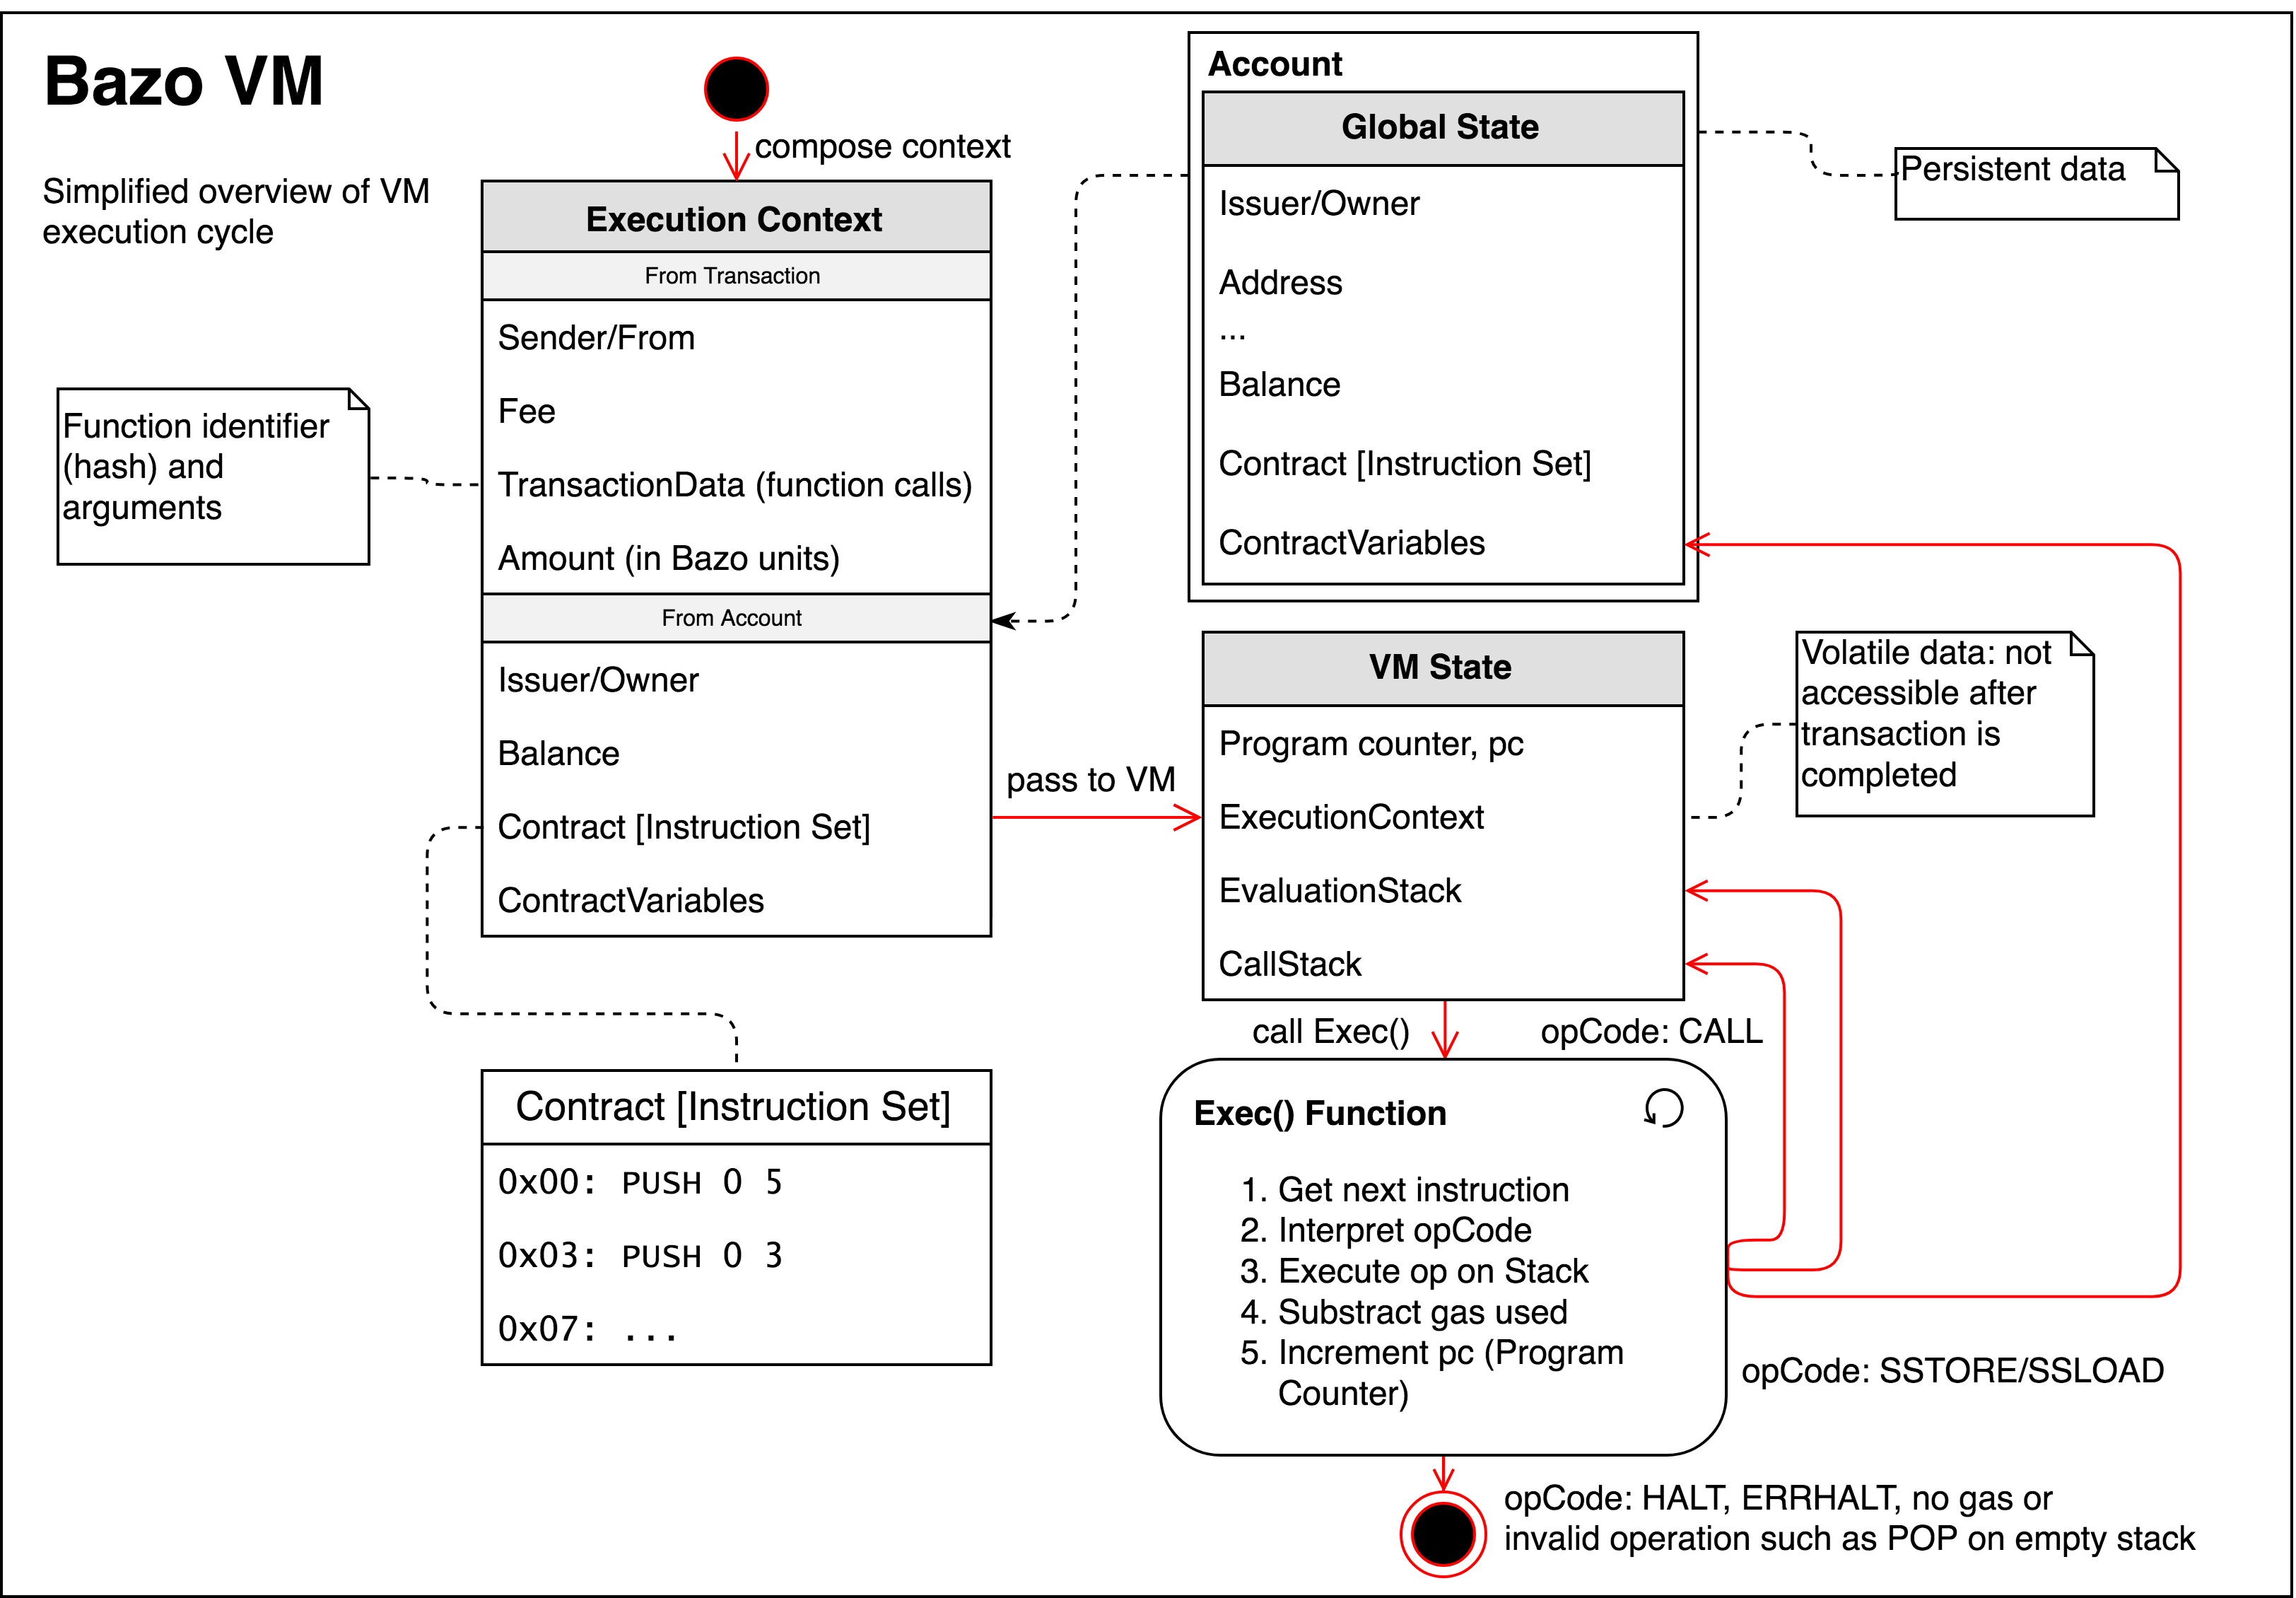
\includegraphics[width=0.84\textwidth]{./images/execution-cycle}
	\caption{Virtual machine execution cycle overview adapted from \cite{eth_yellowpaper} and \cite{exec_graphic}}
	\label{vmexecutioncycle}
	\end{center}
\end{figure}

\subsection{Types of Virtual Machines}
There are two types of virtual machines. On the one hand, there are register based virtual machines. Examples of register based virtual machines are the Lua VM and the Dalvik VM. On the other, there are stack based virtual machines. The Java Virtual Machine and the .NET CLR are both stack based virtual machines. \cite{stackvsregistervm}

\begin{tabular}[t]{ p{3cm} p{12.5cm}}
\raggedright
\textbf{Register based} &
The data structure of where the operands are stored is based on registers of the CPU, therefore the instructions need to contain the addresses (registers) of the operands. This leads to longer instructions. Figure \ref{register vm} shows how adding two number works on a register based virtual machine. \cite{stackvsregistervm} The instruction is \mintinline{tasm}{ADD R1 R3 R2}.
\end{tabular}
\begin{figure}[H]
	\begin{center}
	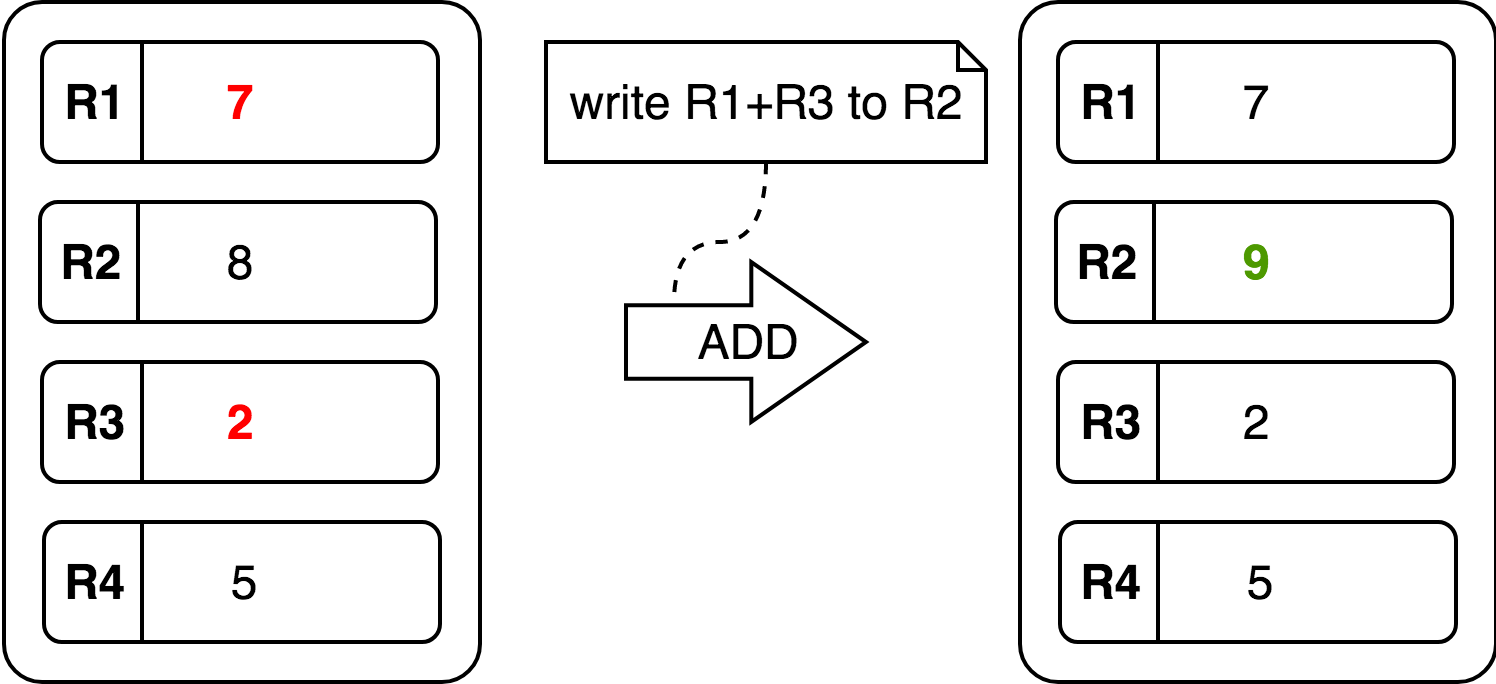
\includegraphics[width=0.61\textwidth]{./images/register-example}
	\caption{Register based virtual machine}
	\label{register vm}
	\end{center}
\end{figure}

\begin{tabular}[t]{ p{3cm} p{12.5cm}}
\raggedright
\textbf{Stack based} &
A stack based virtual machine is based on a LIFO (last in, first out) stack. Operations are carried out by popping and pushing back results on the stack. The main advantage is a stack pointer that implicitly addresses the operands, which means that no addresses are passed in instructions. The instructions set is longer since \mintinline{tasm}{POP} and \mintinline{tasm}{PUSH} instructions have to be included to retrieve and store the operands. \cite{stackvsregistervm} The \gls{instructionset} to add two numbers as shown in figure \ref{stack vm} are: 
\end{tabular}
\begin{figure}[thp]%
    \centering
	\begin{minipage}{0.4\textwidth}
  \begin{minted}	[
	frame=lines,
	framesep=2mm,
	baselinestretch=1.2,
	fontsize=\footnotesize,
	linenos
	]
	{tasm}
	POP
	POP
	ADD
	PUSH
  \end{minted}
  \end{minipage}
  \end{figure}
  \begin{figure}[H]
	\begin{center}
	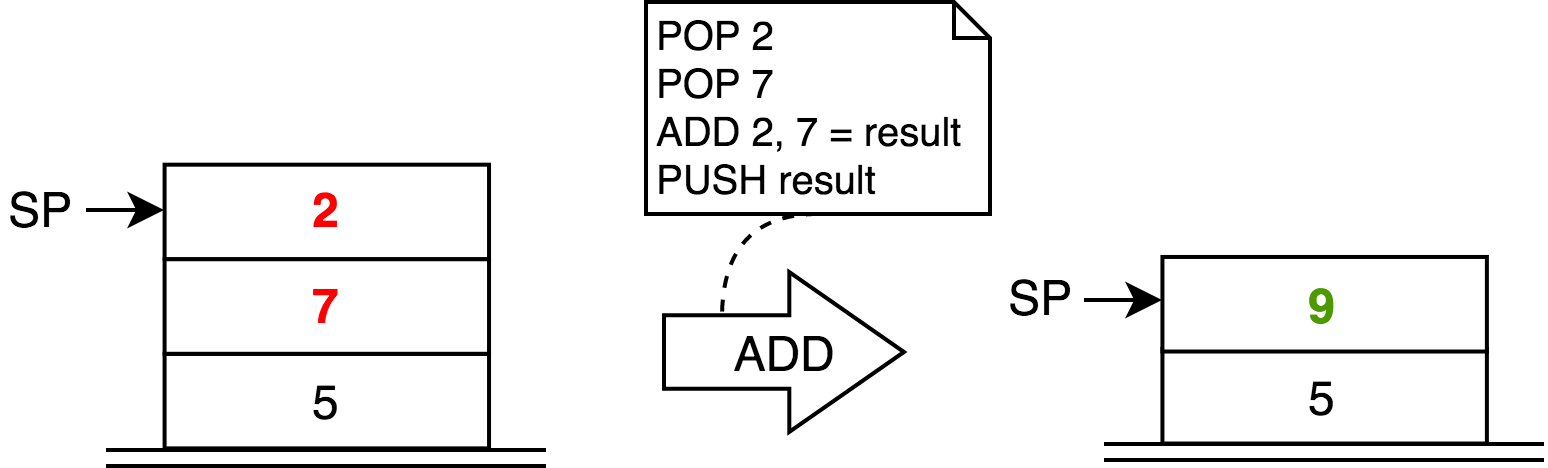
\includegraphics[width=0.6\textwidth]{./images/stack-example}
	\caption{Stack based virtual machine}
	\label{stack vm}
	\end{center}
  \end{figure}

\begin{tabular}[t]{ p{3cm} p{12.5cm}}
\raggedright
\textbf{Design decision} &
Despite the register based virtual machine having advantages such as more possibilities for optimizations and having no overhead from pushing and popping, over a stack based virtual machine, we decided to implement a stack based virtual machine. This decision was most influenced by the implementation of related projects, namely Ethereum and NEO. Besides that, the implementation of a stack based virtual machine is simpler and much more resources are available online.
\end{tabular}

\subsection{Guidelines}
As the Bazo VM continues to be improved or extended by other students, it was paid attention to make the software readable, testable, changeable and extendable. 

\begin{tabular}[t]{ p{3cm} p{12.5cm}}
\raggedright
\textbf{Readability} &
In order to make the code readable code reviews were performed that led to refactorings. \\ \\

\raggedright
\textbf{Testability} &
The code has been written using test driven development, which required writing testable code. In later stages of the project the tests became very useful and made necessary refactorings easier. \\ \\
 
\raggedright
\textbf{Extendability and Changeability} &
The code should be structured and decoupled enough to make necessary changes or extensions to the VM easy for following projects. As described before, having many tests makes the refactoring of the code easier. \\ \\ 
\end{tabular}

\subsection{Notable Design Aspects}
\begin{tabular}[t]{ p{3cm} p{12.5cm}}
\raggedright
\textbf{Fault Tolerance} &
As the VM just executes the instructions it receives without any checks, it could enter an error state and \gls{panic}. It must not be possible to crash the miner with a malicious or erroneous contract. \\ \\

\textbf{Informative Error Messages} &
Throughout the implementation of the VM it was paid attention to write informative error messages, since that simplifies the development of a compiler, which is known to be a follow-up project. Furthermore, the debugging of smart contracts should be easy and streamlined as possible. \\ \\
\end{tabular}

\section{Contract Deployment}

\begin{tabular}[t]{ p{3cm} p{12.5cm}}
\raggedright
\textbf{State of the Art} &
Other blockchains such as Ethereum allow to create and deploy a contract over an IDE. These contracts can be written in a high level language and they can be deployed automatically. In this work the foundation for smart contract deployment and execution has been laid out and designed accordingly. To make it as easy for the end user as mentioned above, a lot more work and resources would have to be invested. \\ \\

\raggedright
\textbf{Current Contract Deployment} &
Currently, contracts are account transactions and as Bazo is permissioned, have to be created with the root key pair. These transactions are added to the unprocessed transactions pool of the miner. When creating the account transaction, the contract and the initial values of the contract have to be provided. The miner then validates the transaction and creates a contract account. \\ \\

\raggedright
\textbf{Restrictions} &
This means that yet only developers can create new contracts. \\ \\

\raggedright
\textbf{Rationale} &
To make contract creation available for account owners, it needs to be possible to create a contract account with any valid key pair of a Bazo account. Also the peer 2 peer package would have to support the features implemented during this work.
Both tasks by themselves would have exceeded the scope of this thesis. \\ \\
\end{tabular}

\section{Execution of a Contract Method}
\begin{tabular}[t]{ p{3cm} p{12.5cm}}
\raggedright
\textbf{State of the Art} &
In other blockchains such as Ethereum, smart contracts can be called via the wallet or the Web API. The results can be checked via API, wallet or block explorer. \\ \\
\raggedright
\textbf{Current Contract Execution} &
In Bazo a transaction which calls a contract has to be added to the unprocessed transactions pool. The miner takes the transaction out of the pool and validates it. If the data field of the transaction is set, the miner will setup the VM context and execute the called function in the VM. After a successful execution, the changed contract variables are written back. \\ \\

\raggedright
\textbf{Restrictions} &
As the features are not yet implemented in the client nor the P2P package, it is not possible to send this kind of transaction via the Web API of the miner. It is also not yet possible to check the result, since smart contracts are not part of the block explorer. \\ \\

\raggedright
\textbf{Rationale} &
Implementing the features in the other applications as well would have exceeded the scope of this work. \\ \\
\end{tabular}

\pagebreak

\section{VM Integration} \label{design_miner}
The VM was integrated into the miner. This section describes the most important aspects of the already existing miner implementation which influenced the integration of the VM and the reasons for the adjustments made to the miner. The section also introduces the VM context which is used to provide data for the VM, gives an overview over the data the VM has access to and the rationale behind the solution with the context.

\subsection{Transaction Types of the Miner} \label{transactionTypes}
In previous works concerning the miner, different transaction types were implemented or extended. Below it is described what the purpose of these transactions is, how they are extended in this work and why they were chosen for extention.

\begin{tabular}[t]{ p{3cm} p{12.5cm}}
\raggedright
\textbf{FundsTx} &
This type of transaction is used to transfer Bazo coins from one account to another and can be used by any externally owned account.\cite{ba_miner} For this reason it was extended with a \textit{Data} field to enable users to call smart contract functions.
\\ \\
\end{tabular}

\begin{figure}[thp]%
    	\centering
		\begin{minipage}{0.4\textwidth}
		\begin{minted}
		[
		frame=lines,
		autogobble,
		framesep=2mm,
		baselinestretch=1.2,
		fontsize=\footnotesize,
		linenos
		]
		{go}
		type FundsTx struct {
			Header byte
			Amount uint64
			Fee    uint64
			TxCnt  uint32
			From   [32]byte
			To     [32]byte
			Sig1   [64]byte
			Sig2   [64]byte
			Data   []byte
		}
		\end{minted}
		\caption{Struct of the type FundsTx}
		\end{minipage}
\end{figure}

\begin{tabular}[t]{ p{3cm} p{12.5cm}}
\raggedright
\textbf{AccTx} &
The account transaction is used to create a new account. As for now, this type of transaction is only allowed to root accounts, since the signature has to be signed with the private key of a root account. \cite{ba_miner} It is important to note that since the miner distinguishes between the transaction types for the corresponding functionality by a switch case in most of its files. \\ \\
\end{tabular}

\begin{tabular}[t]{ p{3cm} p{12.5cm}}
\raggedright
&
It would have been very time consuming to extend the miner by another transaction. Therefore and because most importantly a smart contract needs all fields of an account anyway, it was decided to add the required fields for the contract to the account transaction and leave them set to nil in a normal account transaction. The required fields are \textit{Contract} which stores the code of the contract and \textit{ContractVariables} which contains the state variables. \\ \\
\end{tabular}

\begin{figure}[thp]%
    	\centering
		\begin{minipage}{0.4\textwidth}
		\begin{minted}
		[
		frame=lines,
		autogobble,
		framesep=2mm,
		baselinestretch=1.2,
		fontsize=\footnotesize,
		linenos
		]
		{go}
		type AccTx struct {
			Header            byte
			Issuer            [32]byte
			Fee               uint64
			PubKey            [64]byte
			Sig               [64]byte
			Contract          []byte
			ContractVariables []byteArray
		}
		\end{minted}
		\caption{Struct of the type AccTx}
		\end{minipage}
\end{figure}

\begin{tabular}[t]{ p{3cm} p{12.5cm}}
\raggedright
\textbf{ConfigTx} &
This type of transaction is used to change system parameters such as block size, block interval or minimum fee. No changes to the configuration transaction were necessary. For more information about this transaction type, see the thesis of Livio Sgier \cite{ba_miner}. \\ \\
\textbf{StakeTx} &
Since the Bazo Blockchain is in transition from \gls{pow} to Proof of Stake there is a StakeTx transaction type. This type of transaction is being continuously improved in other works. For more information refer to the theses of Simon Bachmann \cite{ba_pos} and Marc-Alain Chételat \cite{ba_client}.
\end{tabular}

\subsection{Accounts} \label{accounts}
An account is the result of processing an account transaction. Account specifically refers to the object created on the heap of the miner created by an account transaction. Accounts can be modified by a funds transaction. Figure \ref{struct_account} shows the struct for Account.

\begin{figure}[thp]%
    	\centering
		\begin{minipage}{0.6\textwidth}
		\begin{minted}
		[
		frame=lines,
		autogobble,
		framesep=2mm,		baselinestretch=1.2,
		fontsize=\footnotesize,
		linenos
		]
		{go}
		type ByteArray []byte

		type Account struct {
			Address            [64]byte  // 64 Byte
			Issuer             [32]byte  // 32 Byte
			Balance            uint64    // 8 Byte
			TxCnt              uint32    // 4 Byte
			IsStaking          bool      // 1 Byte
			HashedSeed         [32]byte  // 32 Byte
			StakingBlockHeight uint32    // 4 Byte
			Contract           []byte
			ContractVariables  []ByteArray
		}
		\end{minted}
		\caption{Struct of the type Account}
		\label{struct_account}
		\end{minipage}
\end{figure}

\begin{tabular}[t]{ p{3cm} p{12.5cm}}
\raggedright
\textbf{Externally Owned Accounts} &
Externally owned accounts are accounts that are owned by the person who has access to the combination of the public and private key. Having both, the person is able to execute transactions from the account. Externally owned accounts do not have an Issuer, a Contract or ContractVariables. \\ \\
\textbf{Smart Contract Accounts} &
Smart contract accounts are created and owned by externally owned accounts. The field Issuer is set and shows which externally owned account issued the account transaction of the contract account. A smart contract account contains its code in the contract field and if necessary contains its state in contract variables. Contract variables can be altered through contract functions.
\end{tabular}

\subsection{Execution Context}
\begin{tabular}[t]{ p{3cm} p{12.5cm}}
\raggedright
\textbf{Consistency} &
Since the blockchain is a distributed database and the VM needs to change the data of the blockchain eventually, consistency was a very important aspect of its integration. In order to keep the data of the miner consistent even after a potential failure of the VM, the context in which the VM is executed is created by the miner and passed to the VM. This is referred to as execution context. \\ \\ %Especially important hereby is letting the VM only work on copies in order to avoid encapsulation breaches where the VM adjusts a reference values used by the miner directly. If the VM executes without an error the miner writes the changes back by itself. Therefore in the case of an error the copies just have to be discarded, which is a lot easier than resetting the changed variables back to the old values.

\raggedright
\textbf{Content of the Context} &
The execution context is composed with data coming from the transaction and the account. The execution context contains all the data needed to start the execution of the contract. \\ \\ 

\raggedright
\textbf{Access to the Data} &
Specific instructions that get the value from the context and put it on the top of the stack are provided. This for example allows the creation of a contract with functions only the contract issuer can call. In this case, the issuer field is accessed from the contract to verify ownership.
\end{tabular}

\section{Parser}
Since writing all contracts directly in byte code can be very complicated and time-consuming, it was decided to write a very basic parser. The goal of the parser was to make writing contracts easier by allowing the usage of labels and comments. Having labels resolves the problem of counting addresses when using control flow \glspl{opcode} like \mintinline{yaml}{JMP} and \mintinline{yaml}{CALL} since they generally take an address as argument and change the program counter accordingly. The parser could be used as foundation for building a compiler which translates a contract written in a high-level language into \frqq Bazo Byte Code\flqq{}. For the rest of this thesis the code that can be interpreted by the parser is referred to as \flqq Enhanced Bazo Byte Code\frqq{} and the code the virtual machine operates on and which is stored on the blockchain as \flqq Bazo Byte Code\frqq.

\subsection{\flqq Enhanced Bazo Byte Code\frqq}
Figure \ref{basiccontract_design} shows an example of a contract written in \flqq Enhanced Bazo Byte Code\frqq{}. It is possible to have single line comments and inline comments as well, as seen in line 1 and line 5. Comments and empty lines are ignored by the parser. The first word in line is either an opcode or a label, which ends with a colon. Opcodes are optionally followed by arguments. It is predefined what types of arguments an opcode has. The \mintinline{go}{CALL} opcode in line 4 for instance takes a label and a byte as argument.

\begin{figure}[thp]%
    \centering
	\begin{minipage}{0.6\textwidth}
\begin{minted}
[
	frame=lines,
	framesep=2mm,
	baselinestretch=1.2,
	fontsize=\footnotesize,
	linenos
]
{yaml}
# This is a simple program which calls a function
PUSH 55780
PUSH 5
CALL addNums 2
HALT # stops execution

addNums:
LOAD 0
LOAD 1
ADD
RET
\end{minted}
\end{minipage}
\caption{Basic contract with function call written in \flqq Enhanced Bazo Byte Code\frqq{}}
\label{basiccontract_design}
\end{figure}

\subsection{Compile Process}
First the parser splits the contract written in \flqq Enhanced Bazo Byte Code\frqq{} into tokens. A token consists of a token type and a value. The token type represents a kind of lexical unit e.g. opcode, label or a sequence of input characters. The token types are the symbols that are processed by the parser. \cite{aho_compilers:_2007} To get to the \flqq Bazo Byte Code\frqq{} the resulting set is iterated and the token is replaced by the corresponding byte value.

\section{Smart Contracts}
A smart contract consists of an ABI (application binary interface) and one or more callable functions. Smart contracts are deployed by a transaction (AccTx) and executed by a transaction (FundsTx). When someone wants to call a certain function in a smart contract, a special transaction to the public address of the smart contract is executed. The transaction contains an identifier in the data field, so the ABI can match the identifier with the function the caller wants to execute. Arguments passed to that function are also transmitted in that field. Since a transaction is processed simultaneously on all nodes of the network, all functions have to be deterministic.

\subsection{Coding Smart Contracts}
Smart contracts for the NEO blockchain can be developped in C\#, Java, Kotlin, F\# or Python. \cite{neo_whitepaper} There are different ways to create an Ethereum smart contract. There are different high-level programming languages that can be compiled to Ethereum byte code. Solidity has been developed by the Ethereum community and is the industry standard. Solidity is heavily inspired by JavaScript with the idea to attract JavaScript developers to write smart contracts. In this section a simple contract is written once in Solidity and once in \flqq Enhanced Bazo Byte Code\frqq.

\subsubsection{Sample Smart Contact in Solidity}
\begin{figure}[thp]%
    \centering
	\begin{minipage}{0.5\textwidth}
\begin{minted}
[
	frame=lines,
	framesep=2mm,
	baselinestretch=1.2,
	fontsize=\footnotesize,
	linenos
]
{javascript}
contract MyFirstContract {
  uint myData; //State variable

  function set(uint x) public {
    myData = x;
  }

  function add(uint amount) public {
    myData += amount;
  }

  function sub(uint amount) public {
    myData -= amount;
  }

  function get() public constant returns (uint) {
    return myData;
  }
}
\end{minted}
\end{minipage}
\end{figure}

This contract has the state variable myData. Calling the function set() with an uint parameter sets the variable. Calling the function add or sub allows the transaction sender to either add or subtract a certain amount from that variable. In order to call a function a transaction must be executed.

\subsubsection{Sample smart contract in \flqq Enhanced Bazo Byte Code\frqq}
Compiled Smart Contract with ABI would look like this:
\begin{figure}[thp]%
    \centering
	\begin{minipage}{0.7\textwidth}
\begin{minted}
[
	frame=lines,
	framesep=2mm,
	baselinestretch=1.2,
	fontsize=\footnotesize,
	linenos
]
{yaml}
CALLDATA        # Puts the arguments passed to the smart contract
                # and the function hash on top of stack
# ABI:
DUP
PUSH set
EQ
JMPIF set

DUP
PUSH add
EQ
JMPIF add

DUP
PUSH sub
EQ
JMPIF sub

HALT

:set            # set function
SSTORE myData   # stores the variable in ContractVariables
HALT

:add            # add function
POP
SLOAD myData    # loads the variable and puts a local copy on the stack
ADD
SSTORE myData   # overwrites the variable in ContractVariables
HALT

:sub            # sub function
...
\end{minted}
\end{minipage}
\end{figure}

\section{Fee} \label{fee}
\begin{tabular}[t]{ p{3cm} p{12.5cm}}
\raggedright
\textbf{Incentive} &
Running a node in the network carries costs and the node operators want to be compensated. It is also an incentive to get more people to mine blocks because they can earn money by doing so. \\ \\

\raggedright
\textbf{Security Aspects of the Fee} &
Moreover, the fee can be seen as a way to secure the network. The execution of a contract must be deterministic. Since the virtual machine is Turing complete, it is possible to create contracts, which stay in an endless loop causing the network to get stuck and not accepting new transactions. Subtracting gas with the processing of every instruction, the processing of the transaction comes to an end eventually because no more gas is available. \\ \\

\raggedright
\textbf{Fees in other Blockchains} &
In Ethereum and NEO this fee is called gas. Ethereum calculates the cost depending on which instruction is used and uses the smallest unit of its currency. NEO even separates the fee from the actual currency in order to keep the costs of a transaction stable even if the value of the coin itself rises. Bitcoin calculates the cost depending on the size of the transaction. \\ \\

\raggedright
\textbf{Fees in Bazo} &
The fee is expressed in the smallest unit of Bazo coins. The cost of execution vary depending on the complexity of the opcode and depending on the size of the processed elements, since it is possible to work with elements of arbitrary size. Separating fee from the coins of the blockchain was considered. See Chapter \ref{futureworkandconclusions} for more information.
\end{tabular}

